%\documentclass[10pt,a4paper]{report}
\documentclass[11pt,twoside,a4paper]{article}
\usepackage[utf8]{inputenc}
\usepackage{amsmath}
\usepackage{amsfonts}
\usepackage{amssymb}
\usepackage{graphicx}
\usepackage{caption}
\usepackage{subcaption}
\begin{document}
\begin{center}
Image Processing - Pattern recognition and drone controlling with OpenCV",
Gabriel Hidasy, HIRWAAT.PTE
\end{center}

\section{The Problem}
\paragraph {In} the context of this project a drone is an unmanned aerial
vehicle, capable of hover, particularly a Quad-copter.
\paragraph {Drones} can be controlled remotely by a human or by an autonomous
program,this project aims to produce a framework for controlling the drone from
a computer and integrate it with a pattern recognition algorithm to follow the
pattern in a room. This project does not aim to guarantee an stable flight
but the modular nature of it makes it easy to integrate it in another program.

\section{The equipment}
\paragraph {The} quad-copter used in this project is a Parrot AR-Drone 2.0, the
drone has a front facing camera and is controlled by WiFi.
\begin{figure}[hbtp]
  \centering
\begin{subfigure}{.99\textwidth}
  \centering
  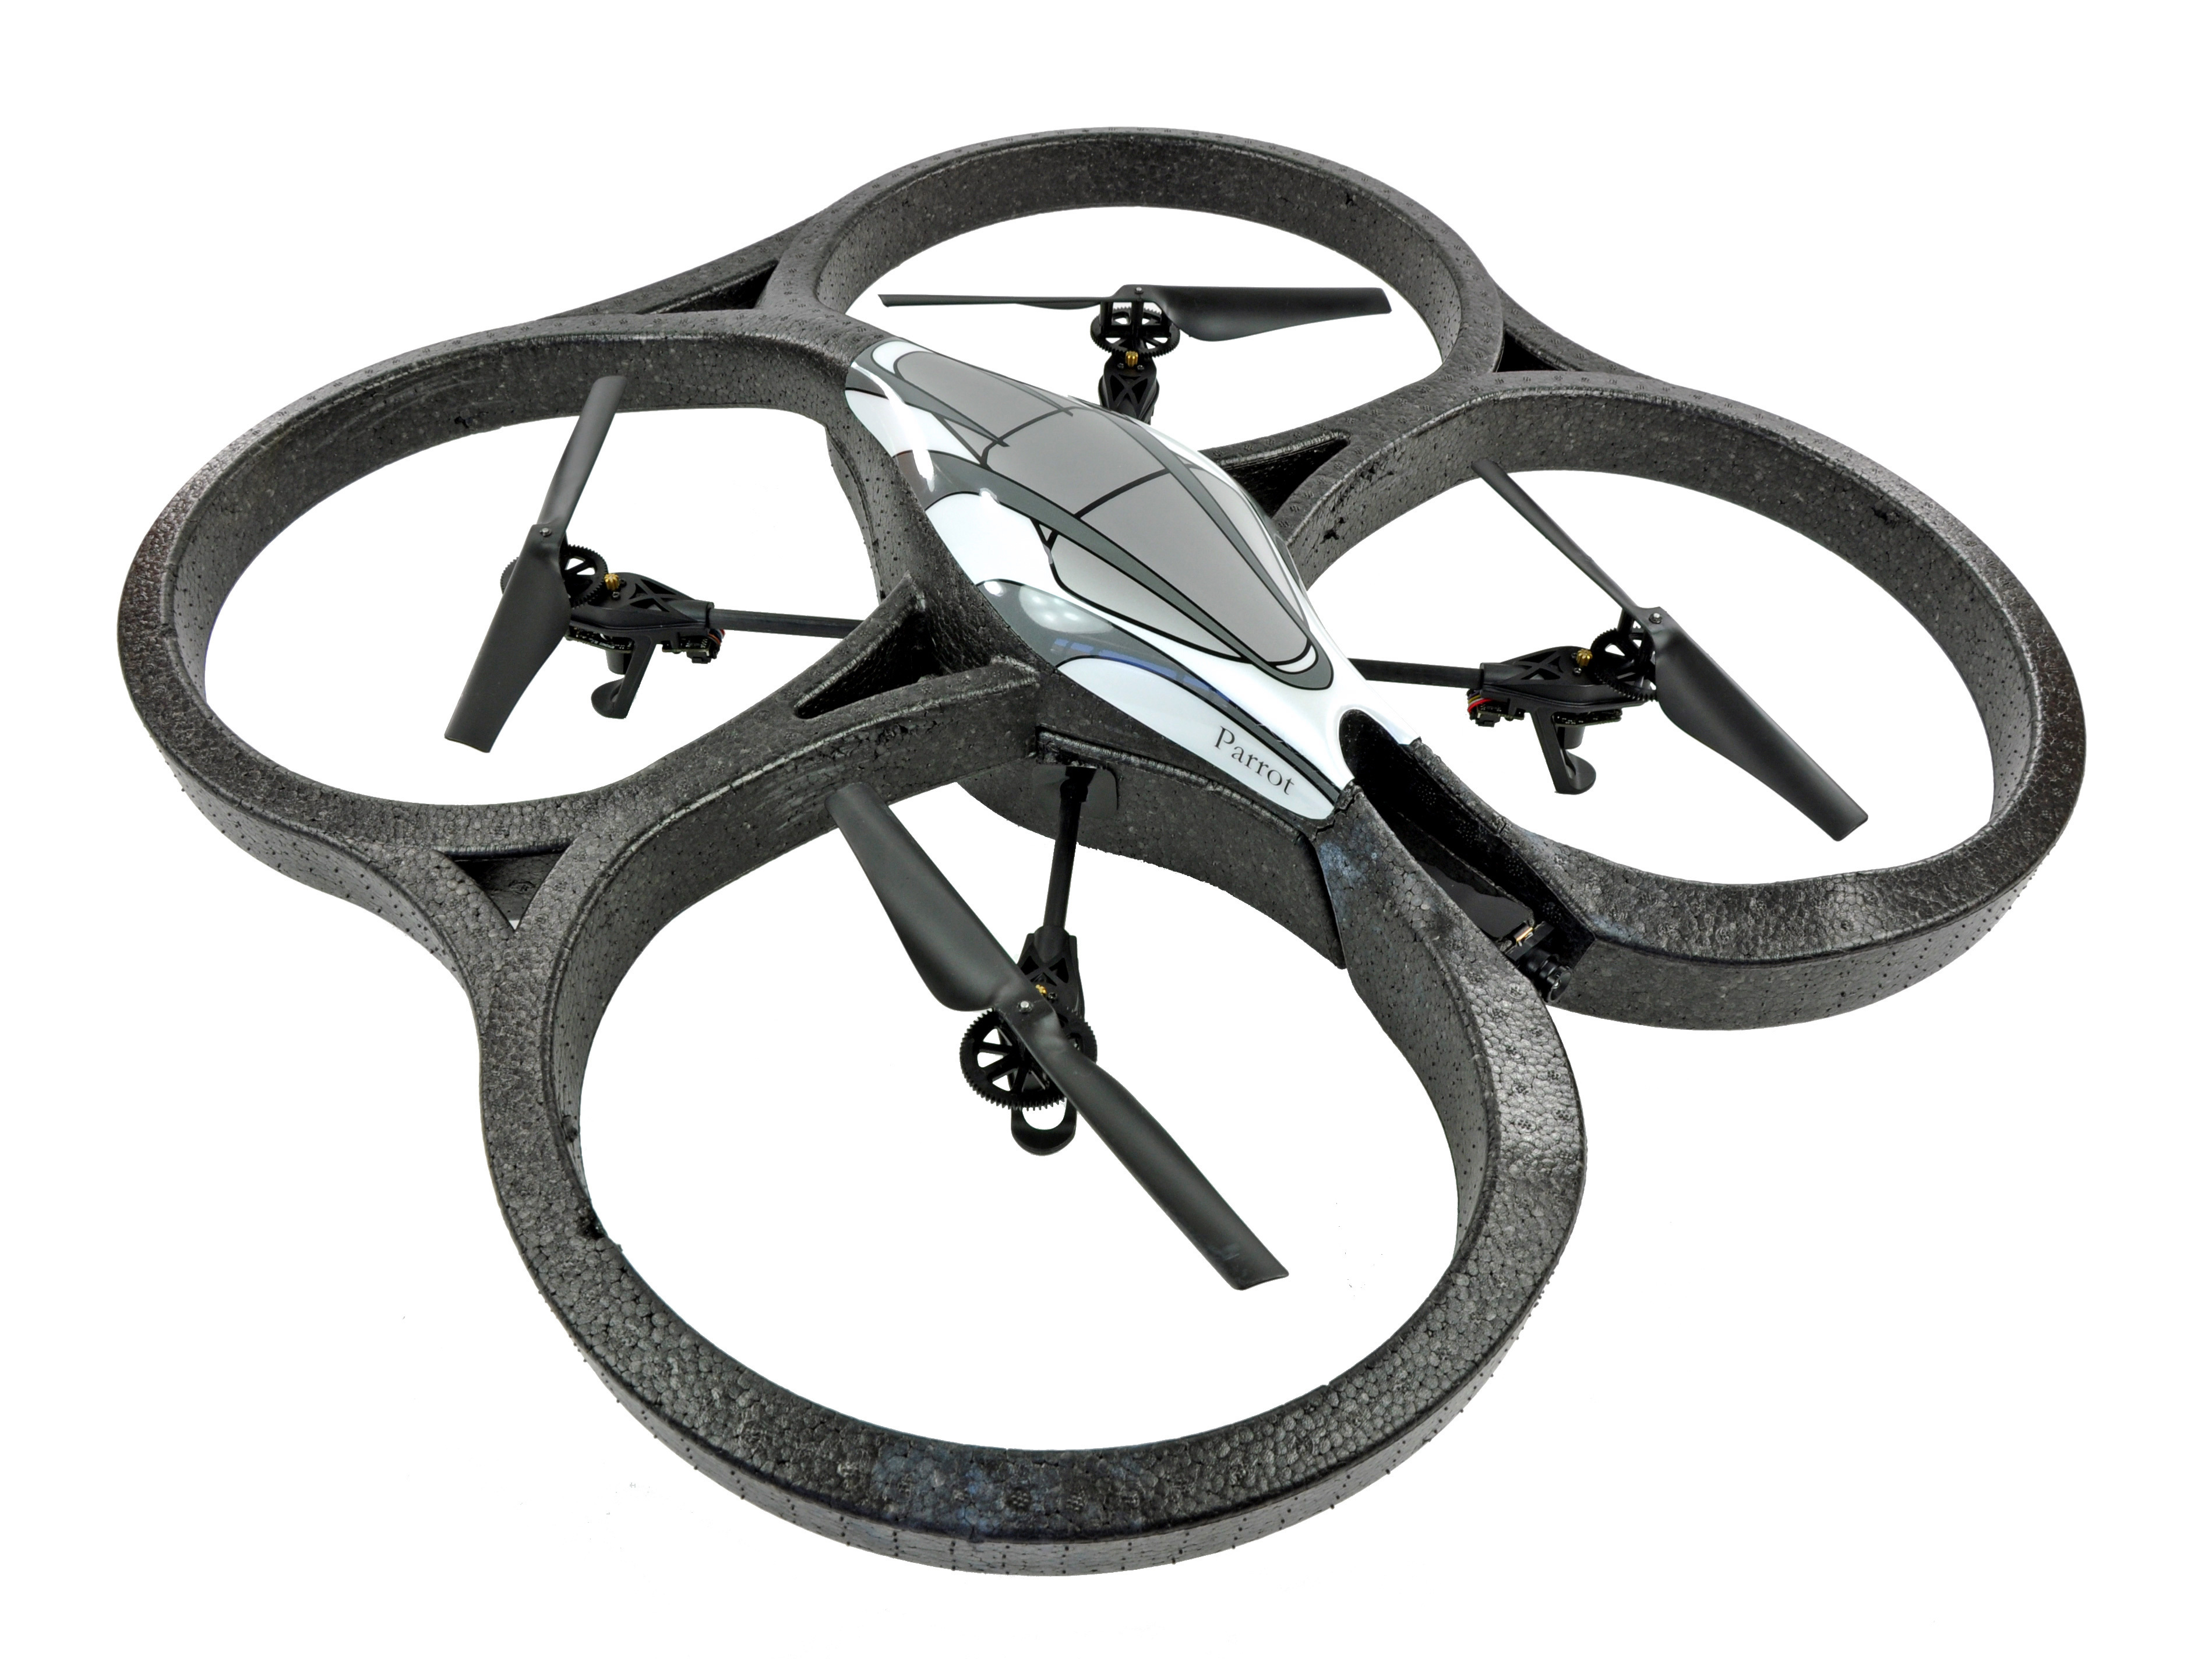
\includegraphics[width=.8\linewidth]{drone.jpg}
\end{subfigure}
\end{figure}

\paragraph {} The controlling application is written in JavaScript and tested
in a notebook and an ARM board (that has the added advantage of being light
enough to be carried by the drone, enabling long range autonomous flights)
\begin{figure}[hbtp]
  \centering
\begin{subfigure}{.99\textwidth}
  \centering
  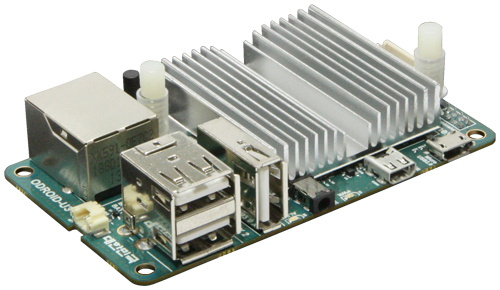
\includegraphics[width=.8\linewidth]{odroid.jpg}
\end{subfigure}
\end{figure}

\section{The solution}
\paragraph {} The solution is divided in 2 independent modules, a controlling
application that communicates with the drone and the pattern matcher that
finds the pattern and gives commands to the controller, this applications
communicate through a web interface and do not need to be hosted in the same
machine.
\paragraph {} The controlling application is based in a NodeJS library that
handles the low level communication, it exports a series of URLs that correspond
to various functions of the drone.\\More then one application can access this
API at a time, there are no security features implemented for now, but it
would not be hard to add an authorization token.
\paragraph {} The functions available in the API are:
\begin{itemize}
\item takeoff
\item land
\item up ([speed, optional, default 0.5],[time, optional, default 500ms])
\item down ([speed, optional, default 0.5],[time, optional, default 500ms])
\item front ([speed, optional, default 0.5],[time, optional, default 500ms])
\item back ([speed, optional, default 0.5],[time, optional, default 500ms])
\item left ([speed, optional, default 0.5],[time, optional, default 500ms])
\item right ([speed, optional, default 0.5],[time, optional, default 500ms])
\item rotatel ([speed, optional, default 0.5],[time, optional, default 500ms])
\item rotater ([speed, optional, default 0.5],[time, optional, default 500ms])
\item stop
\item flip
\item img.jpg (This returns a jpg snapshot from the drone)
\end{itemize}
\paragraph {} The functions are exported by a Web API available by accessing
the URL <IP>:8002/<functionName>. Parameters can be passed by GET or POST, eg:\\
127.0.0.1:8002/up?speed=0.8\&time=100

\paragraph {} The pattern matching application is composed of:
\begin{itemize}
  \item A SURF detector from OpenCV\\
SURF is responsible for finding key-points in an image. A key-point is a point
in the image with some robust feature. A robust feature is a detail of an image
that can be detected even if its scaled, rotated, or slightly deformed.
\begin{figure}[hbtp]
  \centering
\begin{subfigure}{.45\textwidth}
  \centering
  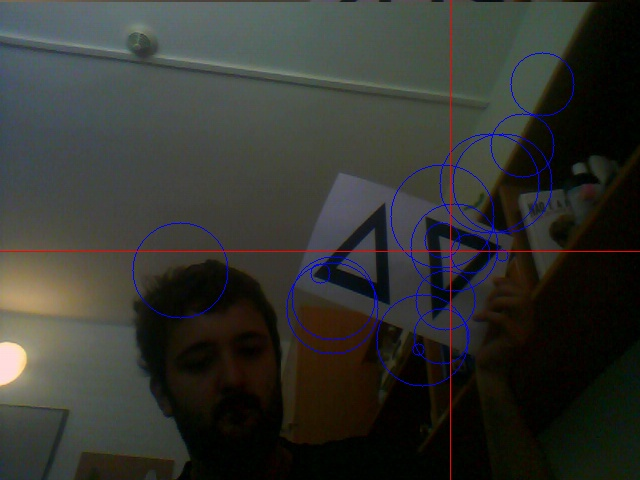
\includegraphics[width=.8\linewidth]{image_marked.jpg}
\end{subfigure}
\begin{subfigure}{.45\textwidth}
  \centering
  
\includegraphics[width=.8\linewidth]{template_marked.jpg}
\end{subfigure}
\end{figure}


%Add a photo of the template and the points, with circles
  \item A FLANN matcher from OpenCV\\
FLANN is a smart algorithm to find matches in a set of data points, it was used
in place of an exhaustive search because, despite not being as accurate, it is
good enough and a lot faster, enabling the algorithm to run in a cheap ARM board
with low power requirements.
\begin{figure}[hbtp]
  \centering
\begin{subfigure}{.99\textwidth}
  \centering
  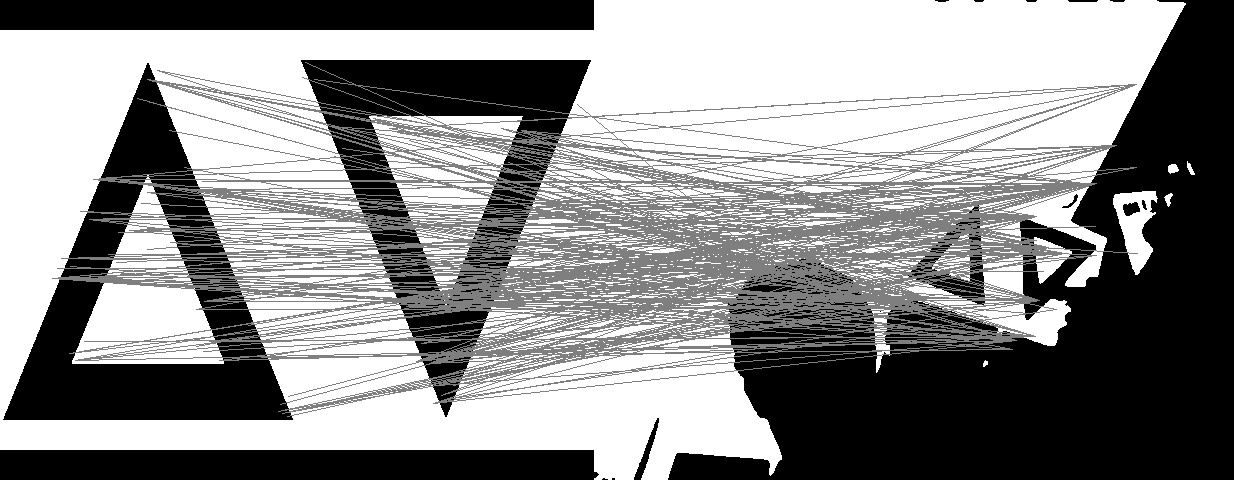
\includegraphics[width=.8\linewidth]{matches.jpg}
\end{subfigure}
\end{figure}
As seem in the image, SURF was applied to a binarized image, this was done as it
reduce problems related to illumination.

  \item A filter: It is possible to see many imperfect matches, they are
filtered out by iteractively removing the points farther away from the gravity
center of the set.

  \item A decision algorithm: A simple algorithm to decide in witch direction
the drone should move based on where the pattern is found (for up, down, left
and right), and the size it appears to have (for front and back), at this
iteration of the project the drone is set to move at only 30\% of its speed
and move for 0.5s at a time.\\
The drone stays still when no pattern is detected, in a future iteration it
could be usefull to have the drone rotating or flying in circles, as it would
increase the chance it would come accross the pattern changing the point of
view.
\end{itemize}


\section{The Results}
\paragraph {} In the following 3 pages a log of a test flight is included, it
consistes of the output from the pattern matcher, to be read as:
\begin{itemize}
\item Date
\item Position (x,y) of the pattern and the geometry of the image
\item Log of commands executed
\end{itemize}
\paragraph{} At this iteration the pattern matcher was not modulating the speed
and time for each function. It was also not commanding the drone to go front or
back.
\newpage
\begin{verbatim}
Wed May 13 14:18:04 CEST 2015
(371, 268, (640,360))
goright
godown
Wed May 13 14:18:05 CEST 2015
(367, 268, (640,360))
godown
Wed May 13 14:18:09 CEST 2015
(322, 205, (640,360))
Wed May 13 14:18:11 CEST 2015
(459, 251, (640,360))
goright
godown
Wed May 13 14:18:13 CEST 2015
(292, 303, (640,360))
godown
Wed May 13 14:18:14 CEST 2015
(456, 262, (640,360))
goright
godown
Wed May 13 14:18:14 CEST 2015
(352, 192, (640,360))
Wed May 13 14:18:15 CEST 2015
(429, 145, (640,360))
goright
Wed May 13 14:18:16 CEST 2015
(468, 115, (640,360))
goright
goup
Wed May 13 14:18:16 CEST 2015
(404, 125, (640,360))
goright
goup
Wed May 13 14:18:17 CEST 2015
(434, 118, (640,360))
goright
goup
Wed May 13 14:18:19 CEST 2015
(412, 133, (640,360))
goright
Wed May 13 14:18:19 CEST 2015
(441, 180, (640,360))
goright
Wed May 13 14:18:20 CEST 2015
(418, 274, (640,360))
goright
godown
Wed May 13 14:18:21 CEST 2015
(425, 217, (640,360))
goright
Wed May 13 14:18:21 CEST 2015
(411, 232, (640,360))
goright
godown
Wed May 13 14:18:22 CEST 2015
(428, 151, (640,360))
goright
Wed May 13 14:18:23 CEST 2015
(408, 183, (640,360))
goright
Wed May 13 14:18:24 CEST 2015
(423, 136, (640,360))
goright
Wed May 13 14:18:25 CEST 2015
(412, 133, (640,360))
(403, 78, (640,360))
goright
goup
Wed May 13 14:18:26 CEST 2015
(367, 81, (640,360))
goup
Wed May 13 14:18:28 CEST 2015
(416, 58, (640,360))
goright
goup
Wed May 13 14:18:29 CEST 2015
(398, 68, (640,360))
goright
goup
Wed May 13 14:18:31 CEST 2015
(406, 58, (640,360))
goright
goup
Wed May 13 14:18:33 CEST 2015
(297, 74, (640,360))
goup
Wed May 13 14:18:33 CEST 2015
(273, 38, (640,360))
goup
Wed May 13 14:18:35 CEST 2015
(312, 52, (640,360))
goup
Wed May 13 14:18:35 CEST 2015
(310, 51, (640,360))
goup
Wed May 13 14:18:36 CEST 2015
(345, 141, (640,360))
Wed May 13 14:18:37 CEST 2015
(422, 167, (640,360))
goright
Wed May 13 14:18:37 CEST 2015
(472, 171, (640,360))
goright
Wed May 13 14:18:38 CEST 2015
(524, 149, (640,360))
goright
Wed May 13 14:18:39 CEST 2015
(523, 200, (640,360))
goright
\end{verbatim}
\newpage
\end{document}
